% !TeX root = ../../main.tex
\subsection{BARCS ranks essential genes as well as general count models in
Cas13 time courses}
\label{sec:liang}

We first tested whether BARCS recovers known biology from a longitudinal
design.  The Cas13 fitness screens of \citet{liang2026lncrna} measured 56,322
guides at days 0, 7, and 14 in five cell lines.  We analyzed HAP1, HEK293FT,
MDA-MB-231, and THP1 and excluded K562, for which one day-0 replicate was not
deposited.  BARCS, official MAGeCK-MLE \citep{li2014mageck}, edgeR-QL
\citep{lun2016edger}, DESeq2 \citep{love2014deseq2}, and limma--voom
\citep{law2014voom} each estimated the same continuous time slope with a
replicate block and two-sided tests.  The deposited values had already
undergone median-of-ratios normalization, ComBat correction, and
replicate-outlier processing, so we rounded them once to the nearest
pseudo-count and supplied the identical matrix to every method.  This analysis
therefore compares methods on a shared processed input, and a test of either
likelihood on raw counts would require the raw reads.

Known essential protein-coding genes served as positives, and targeted lncRNAs
with TPM equal to zero in both available expression assays served as
cell-line-specific proxy nulls.  Limited expression sensitivity and RfxCas13d
collateral activity can place a target with a real fitness effect in this null
set, which rewards conservative methods, so we treat the proxy-null rates as
diagnostics rather than validated type I errors.  To compare calibration on an
equal footing, we assigned the same 1,000 non-targeting guides to 156--159
pseudo-genes per cell line, with guide counts sampled from the target-gene
distribution, and applied one tail-scaling rule to each method's native gene
summary.

All five methods ranked essential genes similarly (Figure~\ref{fig:liang}).
BARCS reached a macro-average precision of 0.876, compared with 0.874 for
edgeR-QL and DESeq2, 0.876 for limma--voom, and 0.877 for MAGeCK-MLE.  At a
gene-level FDR of 0.10, BARCS recovered 0.767 of essential genes in the
depleted direction, the same as limma--voom and more than edgeR-QL (0.746),
DESeq2 (0.758), and MAGeCK-MLE (0.692).  At an empirical 5\% proxy-null
false-positive rate, recall was 0.883 for BARCS and 0.879--0.888 for the
alternatives.  The calibration diagnostics were also similar after the common
scaling rule: the mean absolute calibration error was 0.018 for BARCS and
0.017--0.022 for the alternatives.

Dispersion moderation accounts for this result.  Each guide has only three
residual degrees of freedom in these designs (six libraries and three
coefficients), and without moderation
BARCS reached a precision of 0.838 and an FDR-0.10 recall of 0.600, below all
four alternatives.  Moderation also brought BARCS into closer agreement with
the other guide-level methods.  Among 47,107 proxy-null guides, the number on
which BARCS disagreed with all three of edgeR-QL, DESeq2, and limma--voom fell
from 1,303 to 62, and in every remaining case BARCS was the only method with
$p<0.05$ (Figure~\ref{fig:liang}F--H).

We also asked whether the intermediate time point adds information.  A BARCS
fit using only days 0 and 14 reached a precision of 0.878 and an FDR-0.10
recall of 0.763, compared with 0.876 and 0.767 for the three-time-point fit.
With moderation, the endpoint fit therefore recovered essential genes as
well as the full time course in these screens.  Its value lies in the estimand: the three-time-point fit
estimates a slope over the full course and can be extended to test curvature,
whereas the endpoint fit estimates only the net change.

\begin{figure}[!htbp]
\centering
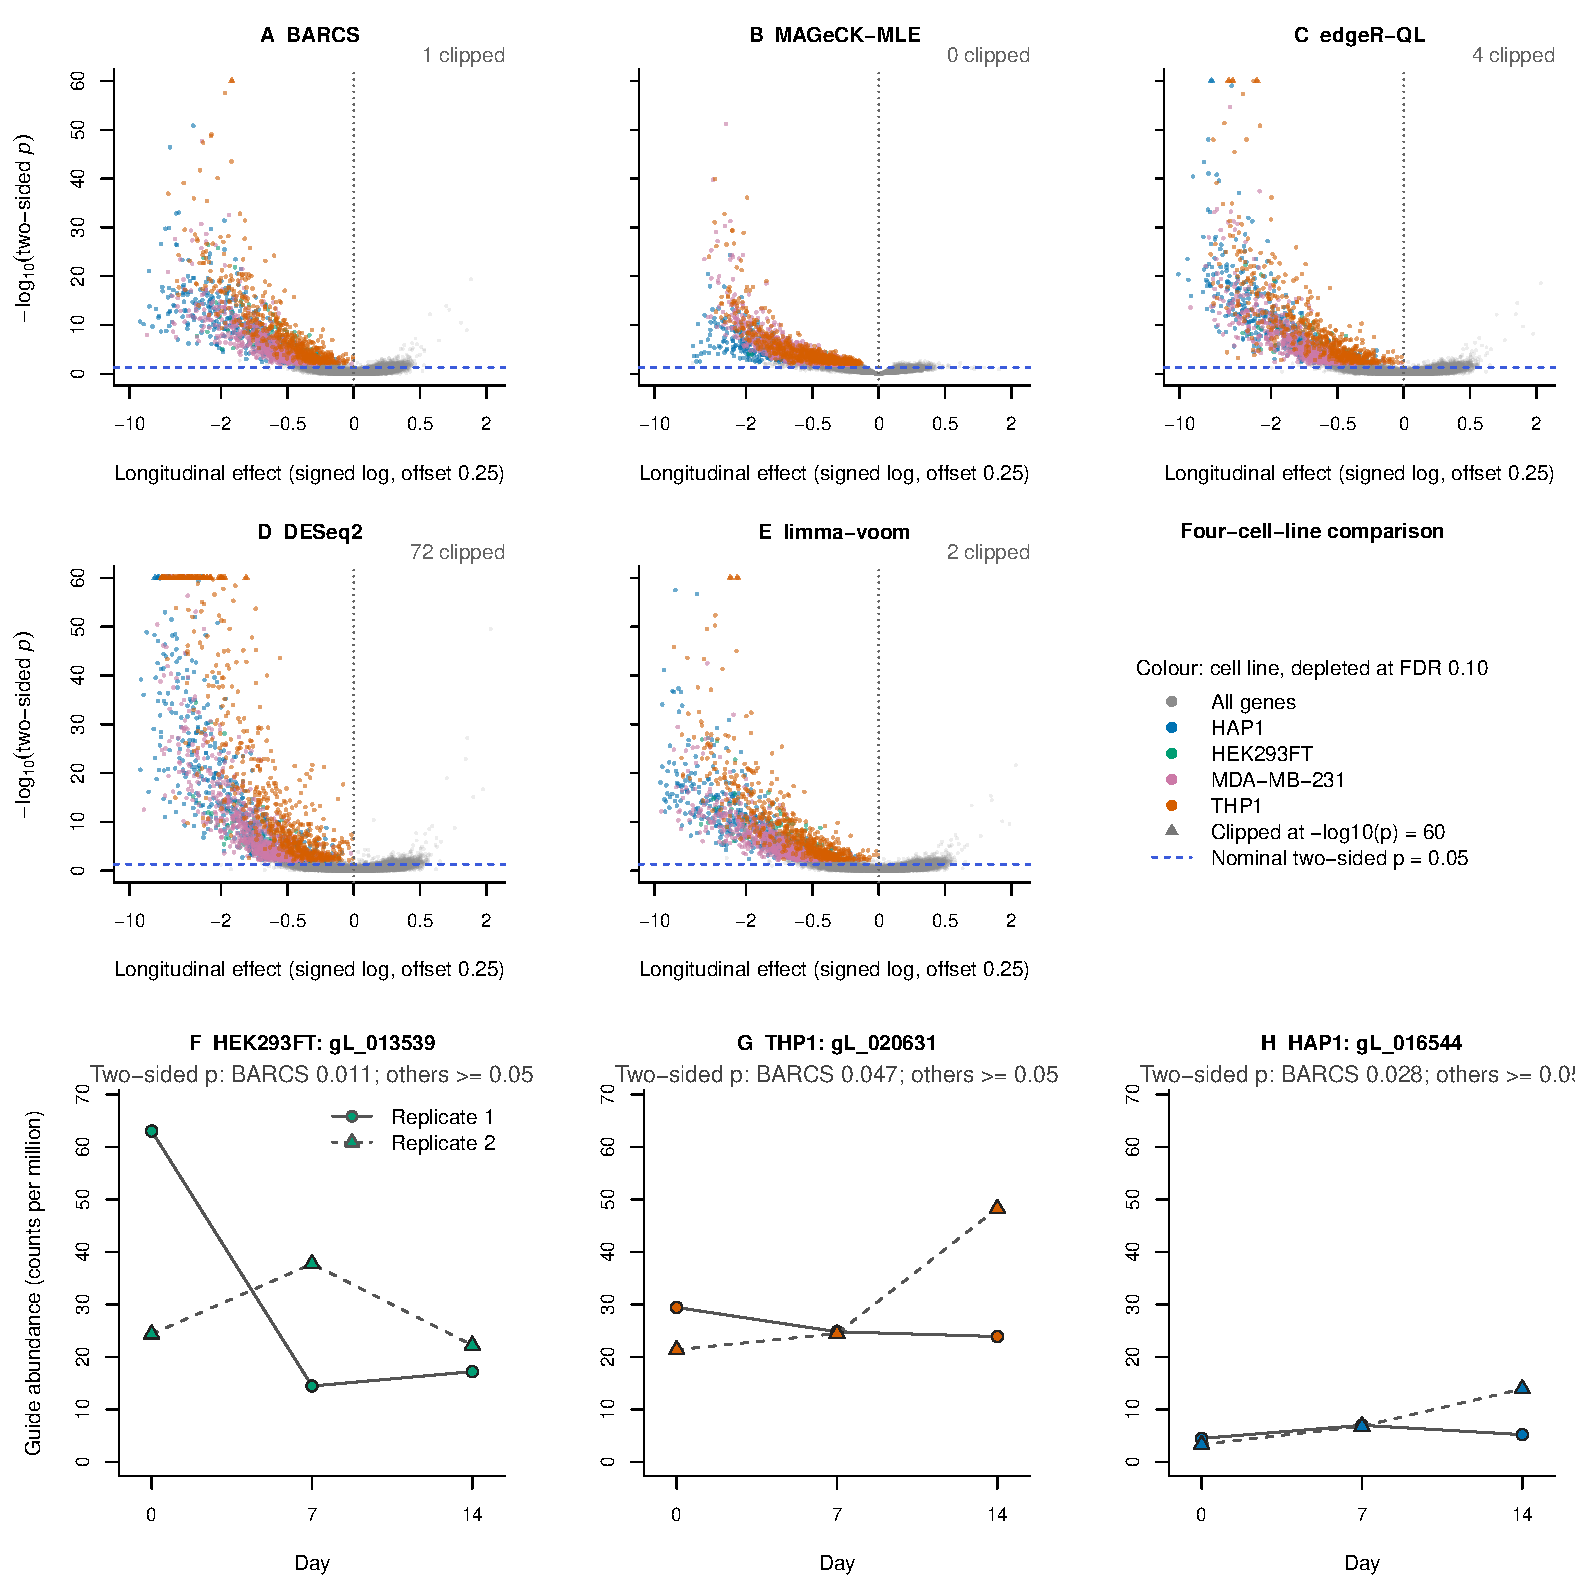
\includegraphics[width=\textwidth]{figures/liang_longitudinal_volcano_trajectories.pdf}
\caption{\textbf{Longitudinal Cas13 analysis using days 0, 7, and 14.}
(A--E) Gene-level results for BARCS, MAGeCK-MLE, edgeR-QL, DESeq2, and
limma--voom across the four replicate-complete cell lines.  All five panels
use common axis scales.  The x axis is the signed logarithmic transform
$\mathrm{sign}(\beta)\log_{10}(1+|\beta|/0.25)$, labelled at the untransformed
effect values.  The horizontal line marks two-sided $p=0.05$, and
$-\log_{10}(p)$ is clipped at 60; triangles mark clipped points, whose count is
shown above each panel.  Colour denotes cell line throughout the figure;
coloured points are negative-effect genes called at FDR 0.10, and all
remaining genes are grey.  (F--H) Processed guide abundance in counts per
million for three proxy-null guides on which BARCS disagreed with all three
other guide-level methods, with markers filled by cell line and replicates
distinguished by point shape and line type.  Among 47,107 proxy-null guides,
62 had BARCS $p<0.05$ while edgeR-QL, DESeq2, and limma--voom all had
$p\geq0.05$, and none showed the opposite pattern (BARCS $p\geq0.20$ with all
three alternatives $p<0.05$).  Within each cell line, the candidate with the
smallest BARCS $p$ was identified, and the three with the largest ratio of the
smallest alternative $p$ to the BARCS $p$ are displayed.  The panels illustrate
the remaining disagreements; they do not estimate their prevalence.}
\label{fig:liang}
\end{figure}

\FloatBarrier
